\documentclass[12pt,tikz]{standalone}
 
\usepackage{tkz-euclide}
\usetikzlibrary{shapes,backgrounds}

\newcommand\Star[3][]{%
		\path[#1] (0  :#3) -- ( 36:#2) 
		-- (72 :#3) -- (108:#2)
		-- (144:#3) -- (180:#2)
		-- (216:#3) -- (252:#2)
		-- (288:#3) -- (324:#2)--cycle;
	}
\newcommand\Center[3][]{
	\begin{scope}[shift = {(#2,#3)}, scale=0.08]
		\Star[#1]{2}{4}
	\end{scope}
	}
	
\newcommand\point[3][]{
	\begin{scope}[shift = {(#2,#3)}, scale=0.08]
		\draw[#1] (0,0) circle (1.5);
	\end{scope}
	}
 
\begin{document}
		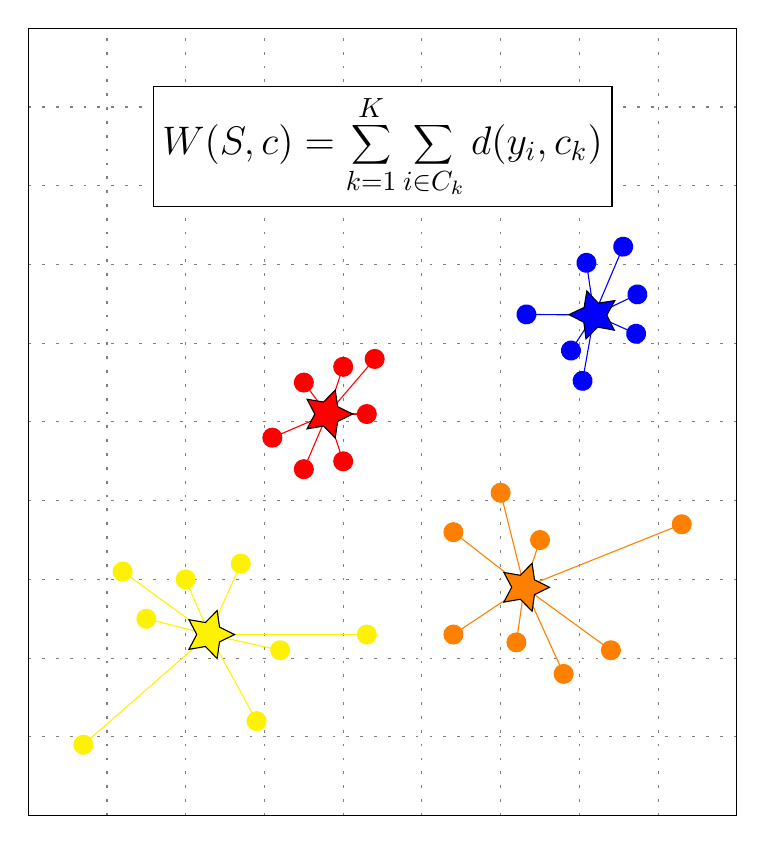
\begin{tikzpicture}[scale=1]
		   \tkzInit[xmax=9,ymax=10,xmin=0,ymin=0]
			\begin{scope}[dash pattern=on 1pt off 4pt]
			\tkzGrid
			\end{scope}
			\draw [draw=black] (0.0,0.0) rectangle (9.0,10.0);
			\node[draw=black, fill=white] at (4.5,8.5) {{\Large$ \displaystyle W(S,c) = \sum_{k=1}^{K}\sum_{i\in C_k}^{} d(y_i,c_k) $}};
			\point[fill=yellow, draw=yellow]{0.7}{0.9}
			\point[fill=yellow, draw=yellow]{2.9}{1.2}`
			\point[fill=yellow, draw=yellow]{3.2}{2.1}			
			\point[fill=yellow, draw=yellow]{4.3}{2.3}
			\point[fill=yellow, draw=yellow]{2.7}{3.2}	
			\point[fill=yellow, draw=yellow]{2}{3}	
			\point[fill=yellow, draw=yellow]{1.2}{3.1}	
			\point[fill=yellow, draw=yellow]{1.5}{2.5}	
			\draw [yellow](2.3,2.3) -- (0.7,0.9);
			\draw [yellow](2.3,2.3) -- (2.9,1.2);
			\draw [yellow](2.3,2.3) -- (3.2,2.1);
			\draw [yellow](2.3,2.3) -- (4.3,2.3);
			\draw [yellow](2.3,2.3) -- (2.7,3.2);
			\draw [yellow](2.3,2.3) -- (2,3);
			\draw [yellow](2.3,2.3) -- (1.2,3.1);
			\draw [yellow](2.3,2.3) -- (1.5,2.5);
			\Center[fill=yellow, draw]{2.3}{2.3}
			
	
			\point[fill=orange, draw=orange]{5.4}{2.3}
			\point[fill=orange, draw=orange]{6.2}{2.2}
			\point[fill=orange, draw=orange]{6.8}{1.8}			
			\point[fill=orange, draw=orange]{7.4}{2.1}
			\point[fill=orange, draw=orange]{8.3}{3.7}	
			\point[fill=orange, draw=orange]{6.0}{4.1}	
			\point[fill=orange, draw=orange]{5.4}{3.6}	
			\point[fill=orange, draw=orange]{6.5}{3.5}	
			\draw [orange](6.3,2.9) --(5.4,2.3);
			\draw [orange](6.3,2.9) --(6.2,2.2);
			\draw [orange](6.3,2.9) --(6.8,1.8);
			\draw [orange](6.3,2.9) --(7.4,2.1);
			\draw [orange](6.3,2.9) --(8.3,3.7);
			\draw [orange](6.3,2.9) --(6.0,4.1);
			\draw [orange](6.3,2.9) --(5.4,3.6);
			\draw [orange](6.3,2.9) --(6.5,3.5);
			\Center[fill=orange, draw]{6.3}{2.9}	
			
			
			\point[fill=red, draw=red]{3.5}{5.5}
			\point[fill=red, draw=red]{4.4}{5.8}
			\point[fill=red, draw=red]{3.5}{4.4}			
			\point[fill=red, draw=red]{3.1}{4.8}
			\point[fill=red, draw=red]{4.0}{5.7}	
			\point[fill=red, draw=red]{4.3}{5.1}		
			\point[fill=red, draw=red]{4.0}{4.5}
			\draw [red](3.8,5.1) --(3.5,5.5);
			\draw [red](3.8,5.1) --(4.4,5.8);
			\draw [red](3.8,5.1) --(3.5,4.4);
			\draw [red](3.8,5.1) --(3.1,4.8);
			\draw [red](3.8,5.1) --(4.0,5.7);
			\draw [red](3.8,5.1) --(4.3,5.1);
			\draw [red](3.8,5.1) --(4.0,4.5);			
			
			\Center[fill=red, draw]{3.8}{5.1}	
			
			\begin{scope}[xshift=7cm, rotate=35]
				\point[fill=blue, draw=blue]{3.1}{5.6}
				\point[fill=blue, draw=blue]{4.1}{5.7}
				\point[fill=blue, draw=blue]{3.2}{4.5}			
				\point[fill=blue, draw=blue]{3.3}{4.9}
				\point[fill=blue, draw=blue]{4.6}{5.6}	
				\point[fill=blue, draw=blue]{4.4}{5.0}		
				\point[fill=blue, draw=blue]{4.1}{4.6}
				\draw [blue](3.8,5.1) --(3.1,5.6);
				\draw [blue](3.8,5.1) --(4.1,5.7);
				\draw [blue](3.8,5.1) --(3.2,4.5);
				\draw [blue](3.8,5.1) --(3.3,4.9);
				\draw [blue](3.8,5.1) --(4.6,5.6);
				\draw [blue](3.8,5.1) --(4.4,5.0);
				\draw [blue](3.8,5.1) --(4.1,4.6);			
				
				\Center[fill=blue, draw]{3.8}{5.1}	
			\end{scope}
			
			
		\end{tikzpicture}
\end{document}